\documentclass[tikz,border=8pt]{standalone}
\usepackage{pgfplots}
\pgfplotsset{compat=1.18}
\definecolor{chapterteal}{HTML}{196F6B}
\definecolor{chapterrust}{HTML}{A3472F}
\definecolor{chaptergold}{HTML}{C58B18}

\begin{document}

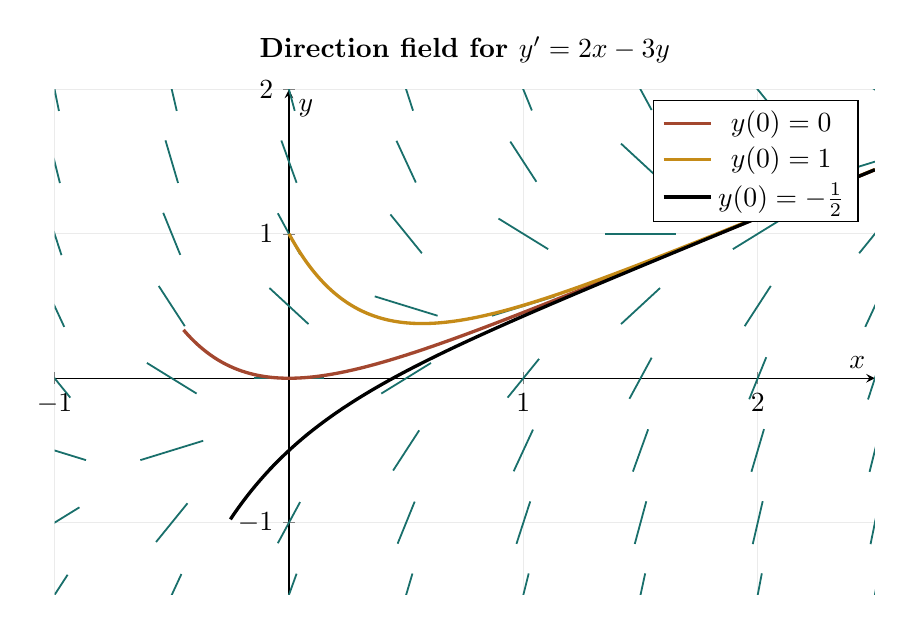
\begin{tikzpicture}
\begin{axis}[
  width=12cm,
  height=8cm,
  axis lines=middle,
  xmin=-1,
  xmax=2.5,
  ymin=-1.5,
  ymax=2,
  xtick={-1,0,1,2},
  ytick={-1,0,1,2},
  xlabel={$x$},
  ylabel={$y$},
  title={Direction field for $y'=2x-3y$},
  title style={font=\bfseries},
  grid=major,
  grid style={black!8},
  clip=true
]
\foreach \x in {-1,-0.5,...,2.5}{
  \foreach \y in {-1.5,-1,...,2}{
    \pgfmathsetmacro{\m}{2*\x-3*\y}
    \pgfmathsetmacro{\dx}{0.15/sqrt(1+\m*\m)}
    \pgfmathsetmacro{\dy}{\m*\dx}
    \pgfmathsetmacro{\xa}{\x-\dx}
    \pgfmathsetmacro{\ya}{\y-\dy}
    \pgfmathsetmacro{\xb}{\x+\dx}
    \pgfmathsetmacro{\yb}{\y+\dy}
    \edef\segment{\noexpand\draw[chapterteal,line width=0.65pt]
      (axis cs:\xa,\ya) -- (axis cs:\xb,\yb);}
    \segment
  }
}
\addplot[chapterrust,very thick,domain=-0.45:2.5,samples=180]
  {0.6666667*x-0.2222222+0.2222222*exp(-3*x)};
\addplot[chaptergold,very thick,domain=0:2.5,samples=180]
  {0.6666667*x-0.2222222+1.2222222*exp(-3*x)};
\addplot[black,very thick,domain=-0.25:2.5,samples=180]
  {0.6666667*x-0.2222222-0.2777778*exp(-3*x)};
\addlegendentry{$y(0)=0$}
\addlegendentry{$y(0)=1$}
\addlegendentry{$y(0)=-\frac12$}
\end{axis}
\end{tikzpicture}

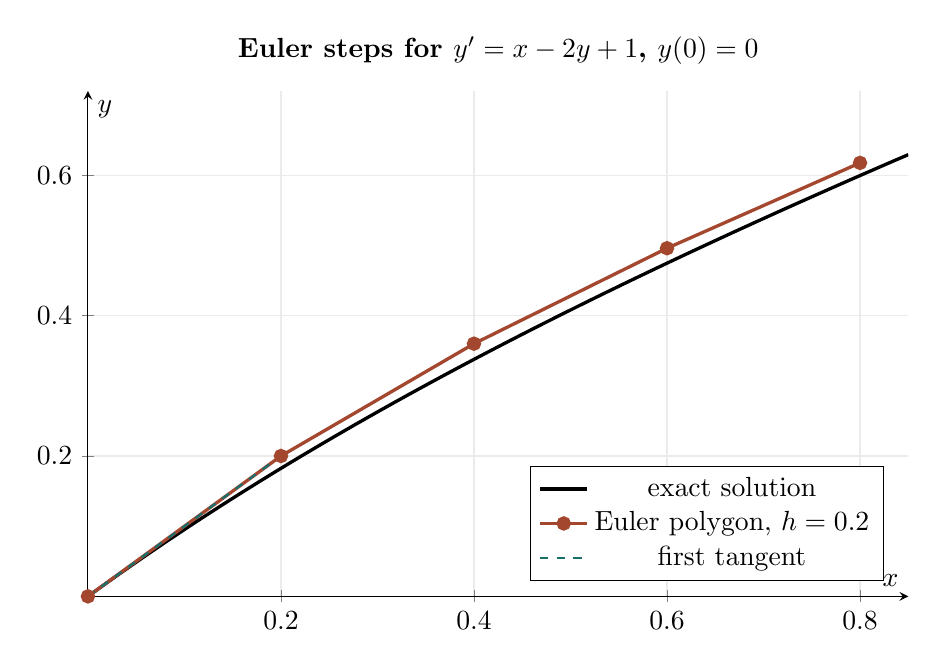
\begin{tikzpicture}
\begin{axis}[
  width=12cm,
  height=8cm,
  axis lines=middle,
  xmin=0,
  xmax=0.85,
  ymin=0,
  ymax=0.72,
  xtick={0,0.2,0.4,0.6,0.8},
  ytick={0,0.2,0.4,0.6},
  xlabel={$x$},
  ylabel={$y$},
  title={Euler steps for $y'=x-2y+1$, $y(0)=0$},
  title style={font=\bfseries},
  grid=major,
  grid style={black!8},
  legend pos=south east
]
\addplot[black,very thick,domain=0:0.85,samples=180]
  {0.5*x+0.25-0.25*exp(-2*x)};
\addlegendentry{exact solution}
\addplot[chapterrust,very thick,mark=*,mark options={fill=chapterrust}]
  coordinates {(0,0) (0.2,0.2) (0.4,0.36) (0.6,0.496) (0.8,0.6176)};
\addlegendentry{Euler polygon, $h=0.2$}
\addplot[chapterteal,dashed,thick,domain=0:0.2] {x};
\addlegendentry{first tangent}
\end{axis}
\end{tikzpicture}

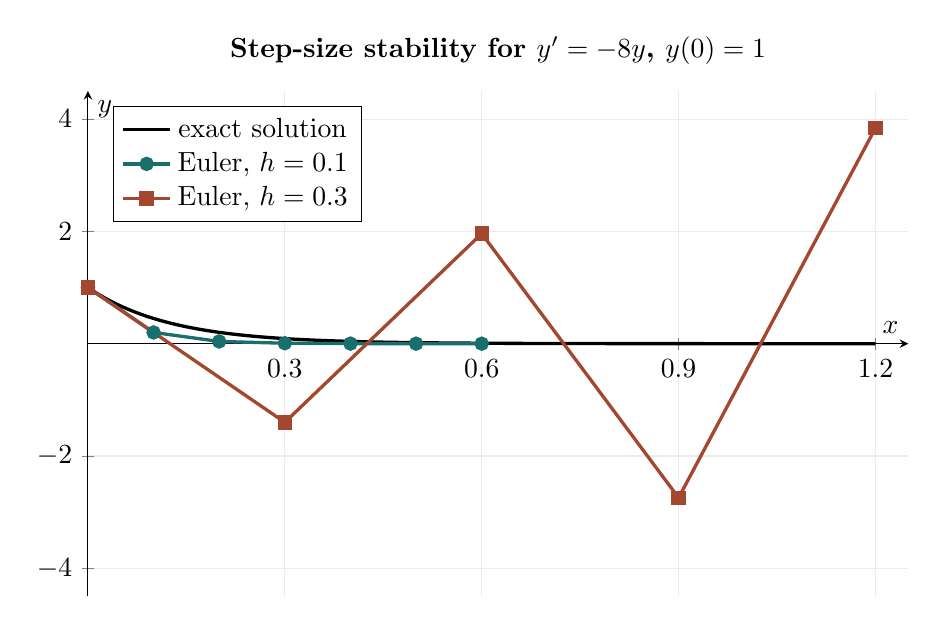
\begin{tikzpicture}
\begin{axis}[
  width=12cm,
  height=8cm,
  axis lines=middle,
  xmin=0,
  xmax=1.25,
  ymin=-4.5,
  ymax=4.5,
  xtick={0,0.3,0.6,0.9,1.2},
  ytick={-4,-2,0,2,4},
  xlabel={$x$},
  ylabel={$y$},
  title={Step-size stability for $y'=-8y$, $y(0)=1$},
  title style={font=\bfseries},
  grid=major,
  grid style={black!8},
  legend pos=north west
]
\addplot[black,very thick,domain=0:1.2,samples=180] {exp(-8*x)};
\addlegendentry{exact solution}
\addplot[chapterteal,very thick,mark=*,mark options={fill=chapterteal}]
  coordinates {(0,1) (0.1,0.2) (0.2,0.04) (0.3,0.008)
  (0.4,0.0016) (0.5,0.00032) (0.6,0.000064)};
\addlegendentry{Euler, $h=0.1$}
\addplot[chapterrust,very thick,mark=square*,mark options={fill=chapterrust}]
  coordinates {(0,1) (0.3,-1.4) (0.6,1.96) (0.9,-2.744) (1.2,3.8416)};
\addlegendentry{Euler, $h=0.3$}
\end{axis}
\end{tikzpicture}

\end{document}
